\chapter{Módulo 2: Evaluación de modelos de aprendizaje automático}

La  evaluación depende de la tarea que se realice. Distinguiremos entre tres tipos de tarea:

\begin{itemize}
    \item \tb{Aprendizaje supervisado}, donde tenemos variables de entrada y una variable de salida, que representa la solución deseada. La meta es aprender la \ti{regla general} que convierte los datos de entrada en la solución correcta. Distinguimos entre:
    \begin{itemize}
        \item \tb{Clasificación}, donde la salida es una categoría.
        \item \tb{Regresión}, la variable resultado es numérica.
    \end{itemize}
    \item \tb{Aprendizaje no supervisado}, no se asigna ninguna etiqueta al algoritmo de aprendizaje, sólo existen variables de entrada. Distinguiremos:
    \begin{itemize}
        \item Clustering
        \item Reglas de asociación, 
        \item Correlaciones
    \end{itemize}
    \item \tb{Aprendizaje de Refuerzo}, donde un programa informático interactúa con un ambiente controlado en el que debe alcanzar una meta concreta: conducir un vehículo o los videojuegos son ejemplos de este tipo de tarea. Muy utilizado en Inteligencia Artificial y/o Robótica.
\end{itemize}

\section{Métricas de Clasificación}

La clasificación se predice a partir de una serie de entradas, para obtener una variable que es \tb{categórica}:
\begin{itemize}
    \item puede tener dos o más valores, 
    \item no tiene un orden, puede ser si/no, a/b/c o d
\end{itemize} 
el modelo lo que intentará predecir a cuál de las clases pertenecen los datos. Lo que tenemos que establecer es que si comparamos la clase predicha y la real coinciden.

La clase predicha se denota como \funcc{h}{x} y la clase actual como \func{x}, donde $x$ es el ejemplo.
\begin{center}
    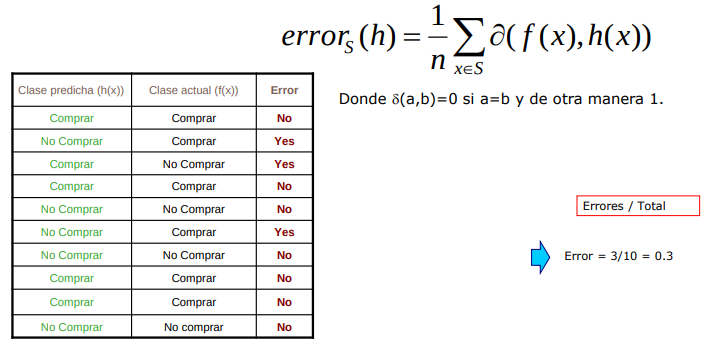
\includegraphics[scale=.65]{images/mod02-01.png}
\end{center}
En el ejemplo, el modelo desplegado, a través de los datos etiquetados como \ti{se ha comprado} o \ti{no se ha comprado} un producto, se comparan con los que predice el modelo. Vemos que en algunos casos no concuerdan, esos casos son \tb{errores}. En la clasificación lo que contamos es cuantas veces se falla, nos estamos refiriendo al \ti{error}; en el ejemplo las veces que falla la predicción son 3 sobre 10, el error es de \nperc{30} o \ti{0.3}. Podemos referirnos de forma inversa y decir que se acierta un \nperc{70} de las predicciones, lo que normalmente se llama \tb{porcentaje de acierto}, en inglés se desgina con el término \tb{accuracy}.

Este tipo de medida, porcentaje de acierto o porcentaje de error, es muy simple y en ocasiones se queda corta a la hora de entender como funciona realmente el modelo.

Una de las métricas habituales en clasificación son las que se conocen como:
\begin{itemize}
    \item \tb{Precission},  representa el porcentaje de documentos que son relevantes para la consulta, con \tb{TP} no referimos a \tb{True Positives}, \ti{valores positivos que han sido verdaderos}, en el ejemplo $TP/ \text{positivos predichos}$.
    ..
    \item \tb{Recall}, representa el porcentaje de documentos que se devuelven por el estudio o modelo (TP ), $TP/ \text{positivos reales}$.
\end{itemize}

Si queremos integrar estados medidas, que nos dé más información, podemos recurrir otro tipo de medida, también habitual que se denomina \tb{Medida F}, o también denominada \tb{media armónica}:

$$\text{Medida F} = 2\,\frac{\text{precission }\ast \text{ recall}}{\text{precission }+ \text{ recall}} = \frac{2TP}{2TP + FP + FN}$$

Un modelo con una \ti{Medida F} alta suele tener medidas altas en precission y recall.

\begin{description}
    \item[TP] o Positivos Predichos correctamente.
    \item[FP]  o Negativos Predichos como Positivos.
    \item[TN] o Negativos Predichos correctamente. 
    \item[FN] o Positivos Predichos como Negativos.  
    \item[TNRate] o porcentaje de negativos verdaderos 
\end{description}
estos parámetros nos permiten conocer el rendimiento de un modelo de clasificación binaria en circunstancias específicas.

\section{Métricas para regresión}

